\section{Evaluation}\label{sec:eval}

\subsection{Aggregated Nonblocking Communication}


\begin{figure}[tbh]
  \begin{center}
  % trimはleft bottom right topの順
  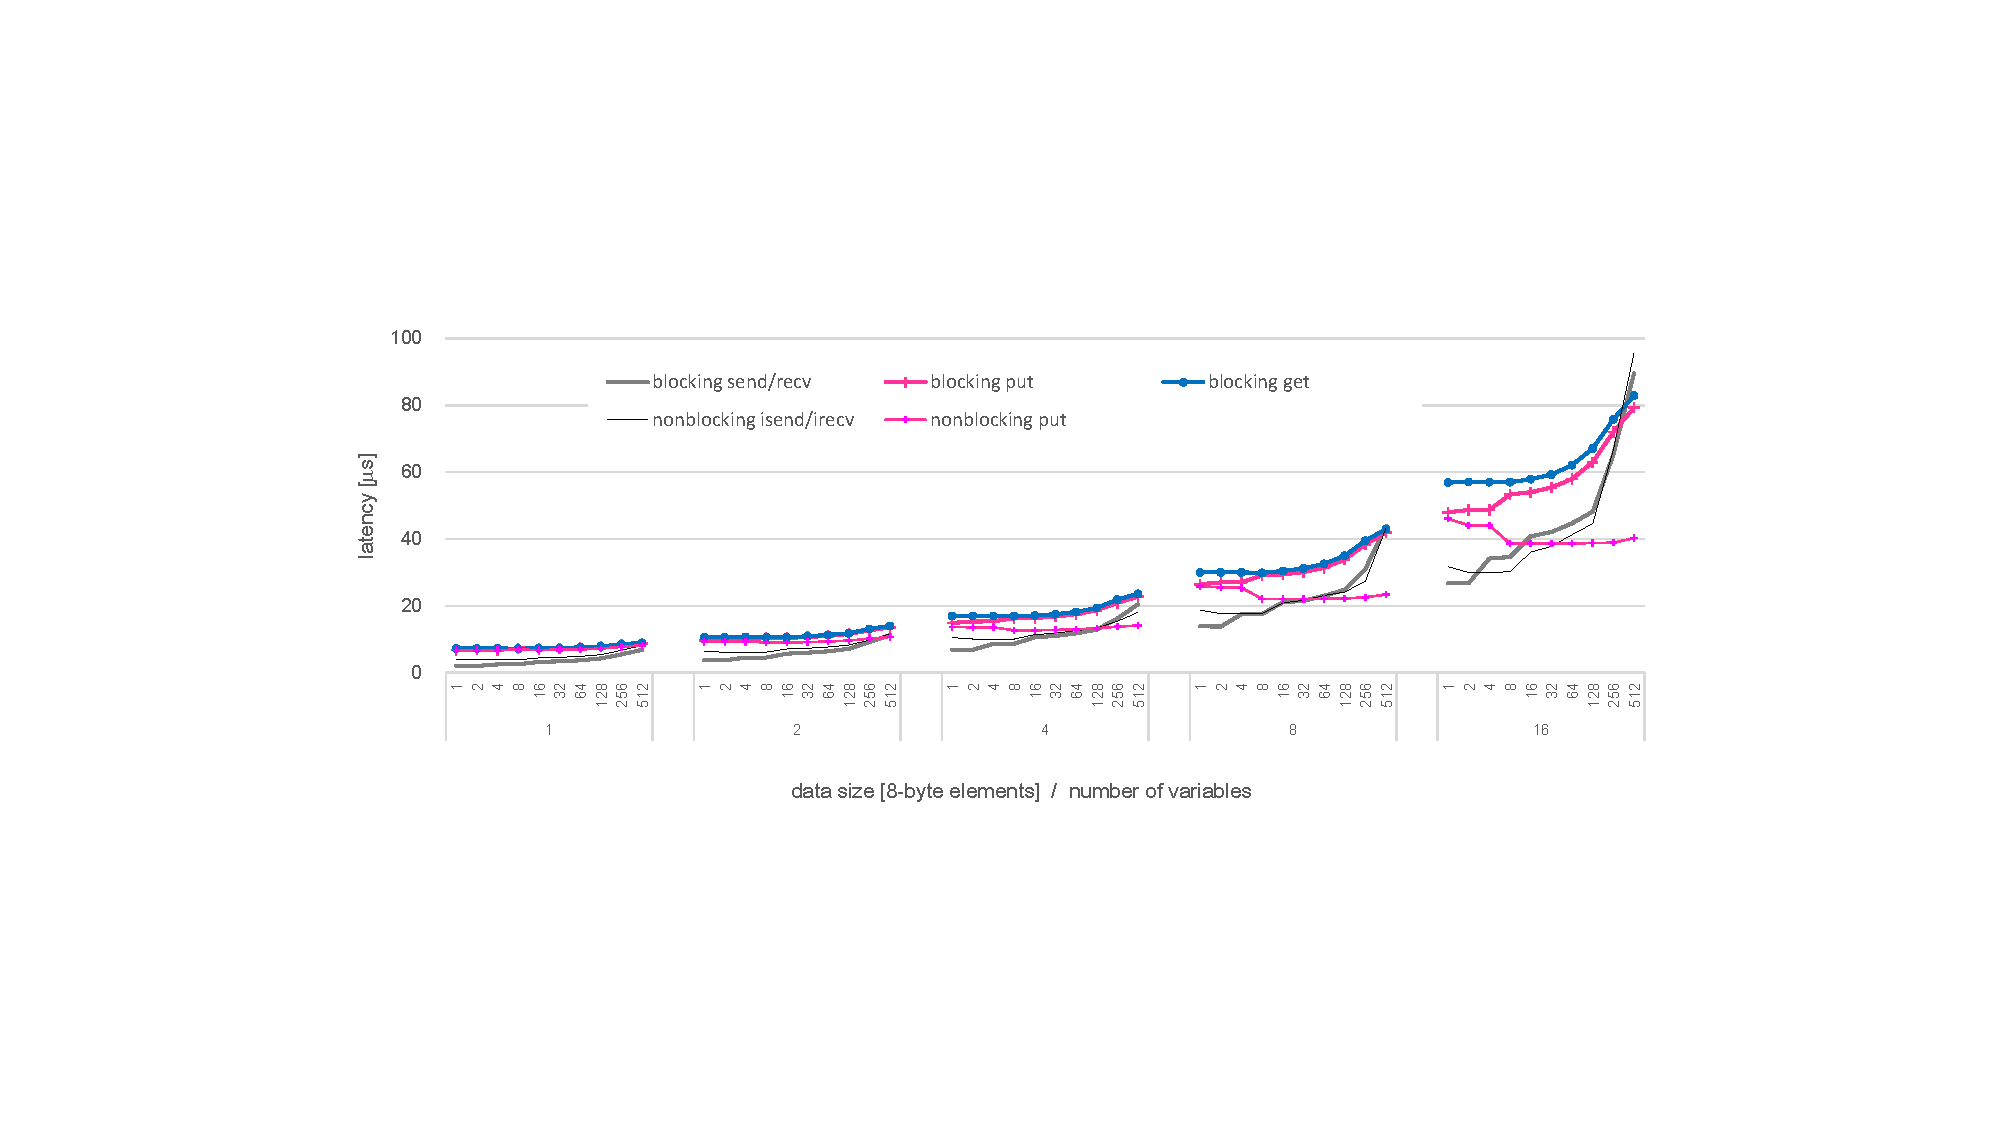
\includegraphics[scale=0.55,trim=6cm 0cm 4cm 6cm,clip]{figs/latency-16var.pdf}

  latency-16var.pdf\\
  2からの4つにして図を大きくする。
  \caption{n-var latency of pingpong}\label{fig:nvar-pp}
  \end{center}
\end{figure}

n-varの効果があった。実際のアプリでもこれはよく起こるパターンである。


\begin{figure}[tbh]
  \begin{center}
  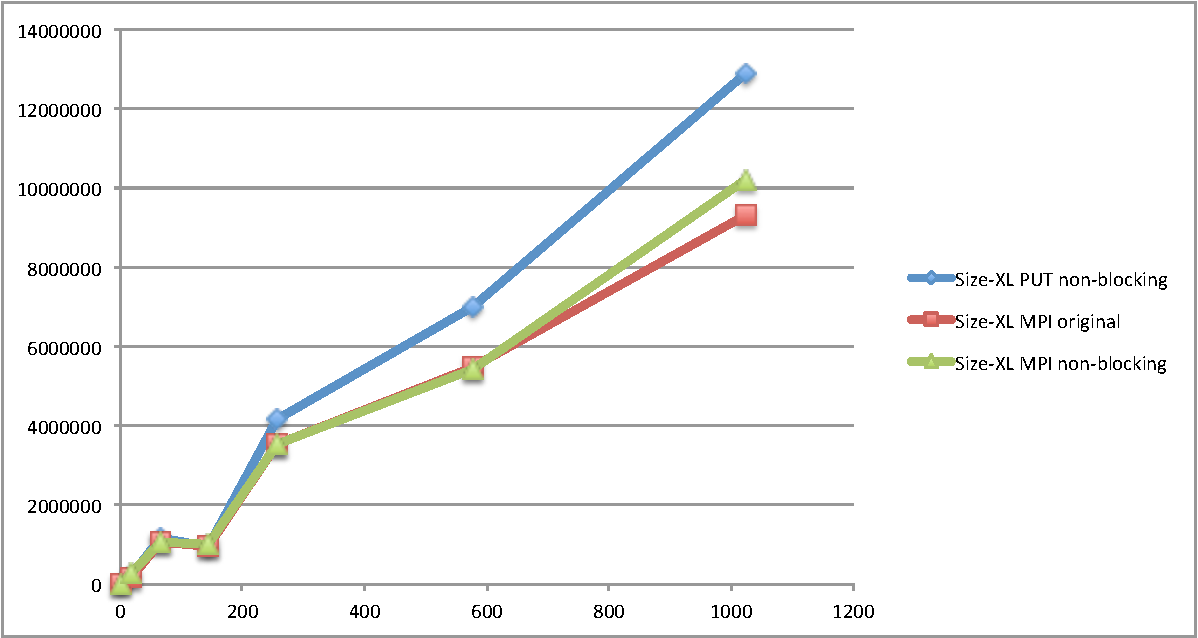
\includegraphics[scale=0.55]{figs/himeno.pdf}

  棒グラフにしてLを加えて2つにするかMまで加えて3つにする

  cf.\ air:/Users/iwashita/Desktop/coarray/Project\_Coarray/coarray\_runtime.pdf

  \caption{Himeno XL}\label{fig:himeno}
  \end{center}
\end{figure}


どういうパターンか分析して説明。n個のcontiguousなnonblocking comm.

